%%%%%%%%%%%%%%%%%%%%%%%%%%%%%%%%%%%%%%%%%
% Beamer Presentation
% LaTeX Template
% Version 1.0 (10/11/12)
%
% This template has been downloaded from:
% http://www.LaTeXTemplates.com
%
% License:
% CC BY-NC-SA 3.0 (http://creativecommons.org/licenses/by-nc-sa/3.0/)
%
%%%%%%%%%%%%%%%%%%%%%%%%%%%%%%%%%%%%%%%%%

%----------------------------------------------------------------------------------------
%	PACKAGES AND THEMES
%----------------------------------------------------------------------------------------

\documentclass{beamer}

\mode<presentation> {

% The Beamer class comes with a number of default slide themes
% which change the colors and layouts of slides. Below this is a list
% of all the themes, uncomment each in turn to see what they look like.

%\usetheme{default}
%\usetheme{AnnArbor}
%\usetheme{Antibes}
%\usetheme{Bergen}
%\usetheme{Berkeley}
%\usetheme{Berlin}
%\usetheme{Boadilla}
%\usetheme{CambridgeUS}
%\usetheme{Copenhagen}
%\usetheme{Darmstadt}
%\usetheme{Dresden}
%\usetheme{Frankfurt}
%\usetheme{Goettingen}
%\usetheme{Hannover}
%\usetheme{Ilmenau}
%\usetheme{JuanLesPins}
%\usetheme{Luebeck}
\usetheme{Madrid}
%\usetheme{Malmoe}
%\usetheme{Marburg}
%\usetheme{Montpellier}
%\usetheme{PaloAlto}
%\usetheme{Pittsburgh}
%\usetheme{Rochester}
%\usetheme{Singapore}
%\usetheme{Szeged}
%\usetheme{Warsaw}

% As well as themes, the Beamer class has a number of color themes
% for any slide theme. Uncomment each of these in turn to see how it
% changes the colors of your current slide theme.

%\usecolortheme{albatross}
%\usecolortheme{beaver}
%\usecolortheme{beetle}
%\usecolortheme{crane}
%\usecolortheme{dolphin}
%\usecolortheme{dove}
%\usecolortheme{fly}
%\usecolortheme{lily}
%\usecolortheme{orchid}
%\usecolortheme{rose}
%\usecolortheme{seagull}
%\usecolortheme{seahorse}
%\usecolortheme{whale}
%\usecolortheme{wolverine}

%\setbeamertemplate{footline} % To remove the footer line in all slides uncomment this line
%\setbeamertemplate{footline}[page number] % To replace the footer line in all slides with a simple slide count uncomment this line

%\setbeamertemplate{navigation symbols}{} % To remove the navigation symbols from the bottom of all slides uncomment this line
}

\usepackage{graphicx} % Allows including images
\usepackage{booktabs} % Allows the use of \toprule, \midrule and \bottomrule in tables
\usepackage{cool}
\usepackage{amsmath}

\newcommand{\vw}{{\bf v_w}}
\newcommand{\vpi}{{\bf v_{\pi}}}
\newcommand{\bphi}{{\bf \Phi}}
\newcommand{\bb}{{\bf B}_{\pi}}
\newcommand{\bpi}{{\bf \Pi}_{{\bf \Phi}}}
\newcommand{\bmu}{{\bf \mu}_{\pi}}
\newcommand{\bv}{{\bf v}}
\newcommand{\bd}{{\bf D}}
\newcommand{\bw}{{\bf w}}
\newcommand{\bdel}{{\bf \delta_w}}
\DeclareMathOperator*{\argmin}{arg\,min}

\newcounter{sauvegardeenumi}
\newcommand{\asuivre}{\setcounter{sauvegardeenumi}{\theenumi}}
\newcommand{\suite}{\setcounter{enumi}{\thesauvegardeenumi}}

%----------------------------------------------------------------------------------------
%	TITLE PAGE
%----------------------------------------------------------------------------------------

\title[Value Function Geometry]{Value Function Geometry and Gradient TD} % The short title appears at the bottom of every slide, the full title is only on the title page

\author{Ashwin Rao} % Your name
\institute[Stanford] % Your institution as it will appear on the bottom of every slide, may be shorthand to save space
{
Stanford University, ICME
}

\date{\today} % Date, can be changed to a custom date

\begin{document}
\begin{frame}
\titlepage % Print the title page as the first slide
\end{frame}

\begin{frame}
\frametitle{Overview} % Table of contents slide, comment this block out to remove it
\tableofcontents % Throughout your presentation, if you choose to use \section{} and \subsection{} commands, these will automatically be printed on this slide as an overview of your presentation
\end{frame}

\section{Motivation and Notation}

\begin{frame}
\frametitle{Motivation for understanding Value Function Geometry}
\begin{itemize}
\item Helps us better understand transformations of Value Functions (VFs)
\item Across the various DP and RL algorithms
\item Particularly helps when VFs are approximated, esp. with linear approx
\item Provides insights into stability and convergence
\item Particularly when dealing with the ``Deadly Triad''
\item Deadly Triad := [Bootstrapping, Func Approx, Off-Policy]
\item {\bf Leads us to Gradient TD}
\end{itemize}
\end{frame}

\begin{frame}
\frametitle{Notation}
\begin{itemize}
\item Assume state space $\mathcal{S}$ consists of $n$ states: $\{s_1, s_2, \ldots, s_n\}$
\item Action space $\mathcal{A}$ consisting of finite number of actions
\item This exposition extends easily to continuous state/action spaces too
\item This exposition is for a fixed (often stochastic) policy denoted $\pi(a|s)$
\item VF for a policy $\pi$ is denoted as $\vpi: \mathcal{S} \rightarrow \mathbb{R}$
\item $m$ feature functions $\phi_1, \phi_2, \ldots, \phi_m : \mathcal{S} \rightarrow \mathbb{R}$
\item Feature vector for a state $s \in \mathcal{S}$ denoted as ${\bf \phi}(s) \in \mathbb{R}^m$
\item For linear function approximation of VF with weights $\bw = (w_1, w_2, \ldots, w_m)$,
VF $\vw: \mathcal{S} \rightarrow \mathbb{R}$ is defined as:
$$\vw(s) = \bw^T \cdot {\bf \phi}(s) =  \sum_{j=1}^m w_j \cdot \phi_j(s) \mbox{ for any } s \in \mathcal{S}$$
\item $\bmu : \mathcal{S} \rightarrow [0, 1]$ denotes the states' probability distribution under $\pi$ 
\end{itemize}
\end{frame}

\section{Geometric/Vector Space Representation of Value Functions}

\begin{frame}
\frametitle{VF Vector Space and VF Linear Approximations}
\begin{itemize}
\item $n$-dimensional space, with each dim corresponding to a state in $\mathcal{S}$
\item A vector in this space is a specific VF (typically denoted $\bv$): $\mathcal{S} \rightarrow \mathbb{R}$
\item Each dimension's coordinate is the VF for that dimension's state
\item Coordinates of vector $\vpi$ for policy $\pi$ are: $[\vpi(s_1), \vpi(s_2), \ldots, \vpi(s_n)]$
\item Consider $m$ vectors where $j^{th}$ vector is: $[\phi_j(s_1), \phi_j(s_2), \ldots, \phi_j(s_n)]$
\item These $m$ vectors are the $m$ columns of $n \times m$ matrix $\bphi = [\phi_j(s_i)]$
\item Their span represents an $m$-dim subspace within this $n$-dim space
\item Spanned by the set of all $\bw = [w_1, w_2, \ldots, w_m] \in \mathbb{R}^m$
\item Vector $\vw = \bphi \cdot \bw$ in this subspace has coordinates $[\vw(s_1), \vw(s_2), \ldots , \vw(s_n)]$
\item Vector $\vw$ is fully specified by $\bw$ (so we often say $\bw$ to mean $\vw$)
\end{itemize}
\end{frame}

\begin{frame}
\frametitle{Some more notation}
\begin{itemize}
\item Denote $r(s,a)$ as the Expected Reward upon action $a$ in state $s$
\item Denote $p(s,s',a)$ as the probability of transition $s \rightarrow s'$ upon action $a$
\item Define
$${\bf R}_{\pi}(s) = \sum_{a \in \mathcal{A}} \pi(a|s) \cdot r(s,a)$$
$${\bf P}_{\pi}(s,s') = \sum_{a \in \mathcal{A}} \pi(a|s) \cdot p(s,s',a)$$
\item Denote ${\bf R}_{\pi}$ as the vector $[{\bf R}_{\pi}(s_1), {\bf R}_{\pi}(s_2), \ldots, {\bf R}_{\pi}(s_n)]$
\item Denote ${\bf P}_{\pi}$ as the matrix $[{\bf P}_{\pi}(s_i, s_{i'})], 1 \leq i, i' \leq n$ 
\item Denote $\gamma$ as the MDP discount factor
\end{itemize}
\end{frame}

\begin{frame}
\frametitle{Bellman operator $\bb$}
\begin{itemize}
\item Bellman operator $\bb$ for policy $\pi$ operating on VF vector $\bv$ defined as:
$$\bb \bv = {\bf R}_{\pi} + \gamma {\bf P}_{\pi} \cdot \bv$$
\item Note that $\vpi$ is the fixed point of operator $\bb$ (meaning $\bb \vpi = \vpi$)
\item If we start with an arbitrary VF vector $\bv$ and repeatedly apply $\bb$, 
by Contraction Mapping Theorem, we will reach the fixed point $\vpi$
\item This is the Dynamic Programming Policy Evaluation algorithm
\item Monte Carlo without func approx also converges to $\vpi$ (albeit slowly)
\end{itemize}
\end{frame}

\begin{frame}
\frametitle{Projection operator $\bpi$}
\begin{itemize}
\item First we define ``distance'' $d({\bf v_1}, {\bf v_2})$ between VF vectors ${\bf v_1}, {\bf v_2}$
\item Weighted by $\bmu$ across the $n$ dimensions of ${\bf v_1}, {\bf v_2}$
$$d({\bf v_1}, {\bf v_2}) = \sum_{i=1}^n \bmu(s_i) \cdot  ({\bf v_1}(s_i) - {\bf v_2}(s_i))^2 =  ({\bf v_1} - {\bf v_2})^T \cdot \bd \cdot ({\bf v_1} - {\bf v_2})$$
where $\bd$ is the square diagonal matrix consisting of $\bmu(s_i), 1 \leq i \leq n$
\item Projection operator for subspace spanned by $\bphi$ is denoted as $\bpi$
\item $\bpi$ performs an orthogonal projection of VF vector $\bv$ on subspace $\bphi$
\item So we need to minimize $d(\bv, \bpi \bv)$
\item This is a weighted least squares regression with solution:
$$\bw = (\bphi^T \cdot \bd \cdot \bphi)^{-1} \cdot \bphi^T \cdot \bd \cdot \bv$$
\item So, the Projection operator $\bpi$ can be written as:
$$\bpi = \bphi \cdot (\bphi^T \cdot \bd \cdot \bphi)^{-1} \cdot \bphi^T \cdot \bd$$
\end{itemize}
\end{frame}

\begin{frame}
\frametitle{4 VF vectors of interest in the $\bphi$ subspace}
Note: We will refer to the $\bphi$-subspace VF vectors by their weights $\bw$

\begin{enumerate}
\item Projection of $\vpi$: $\bw_{\pi} = \argmin_\bw d(\vpi, \vw)$
\begin{itemize}
\item This is the VF we seek when doing linear function approximation
\item Because it is the VF vector ``closest'' to $\vpi$ in the $\bphi$ subspace
\item Monte-Carlo with linear func approx will (slowly) converge to $\bw_{\pi}$
\end{itemize}

\item Bellman Error (BE)-minimizing: $\bw_{BE} = \argmin_\bw d(\bb \vw, \vw)$
\begin{itemize}
\item This is the solution to a linear system (covered later)
\item In model-free setting, Residual Gradient TD Algorithm (covered later)
\item Cannot learn if we can only access features, and not underlying states
\end{itemize}

\asuivre

\end{enumerate}

\end{frame}

\begin{frame}
\frametitle{4 VF vectors of interest in the $\bphi$ subspace (continued)}
\begin{enumerate}

\suite

\item Projected Bellman Error (PBE)-minimizing: $\bw_{PBE} = \argmin_\bw d((\bpi \cdot \bb) \vw, \vw)$
\begin{itemize}
\item The minimum is 0, i.e., $\bphi \cdot \bw_{PBE}$ is the fixed point of operator $\bpi \cdot \bb$
\item This fixed point is the solution to a linear system (covered later)
\item Alternatively, if we start with an arbitrary $\vw$ and repeatedly apply $\bpi \cdot \bb$, we will converge to $\bphi \cdot \bw_{PBE}$
\item This is a DP-like process with approximation - repeatedly thrown out of the $\bphi$ subspace (applying Bellman operator $\bb$),
followed by landing back in the $\bphi$ subspace (applying Projection operator $\bpi$)
\item In model-free setting, Gradient TD Algorithms (covered later)
\end{itemize}

\item Temporal Difference Error (TDE)-minimizing: ${\bf w}_{TDE} = \argmin_w \mathbb{E}_{\pi} [\delta^2]$
\begin{itemize}
\item $\delta$ is the TD error
\item Minimizes the expected square of the TD error when following policy $\pi$
\item Naive Residual Gradient TD Algorithm (covered later)
\end{itemize}

\end{enumerate}
\end{frame}

\begin{frame}
\begin{figure}
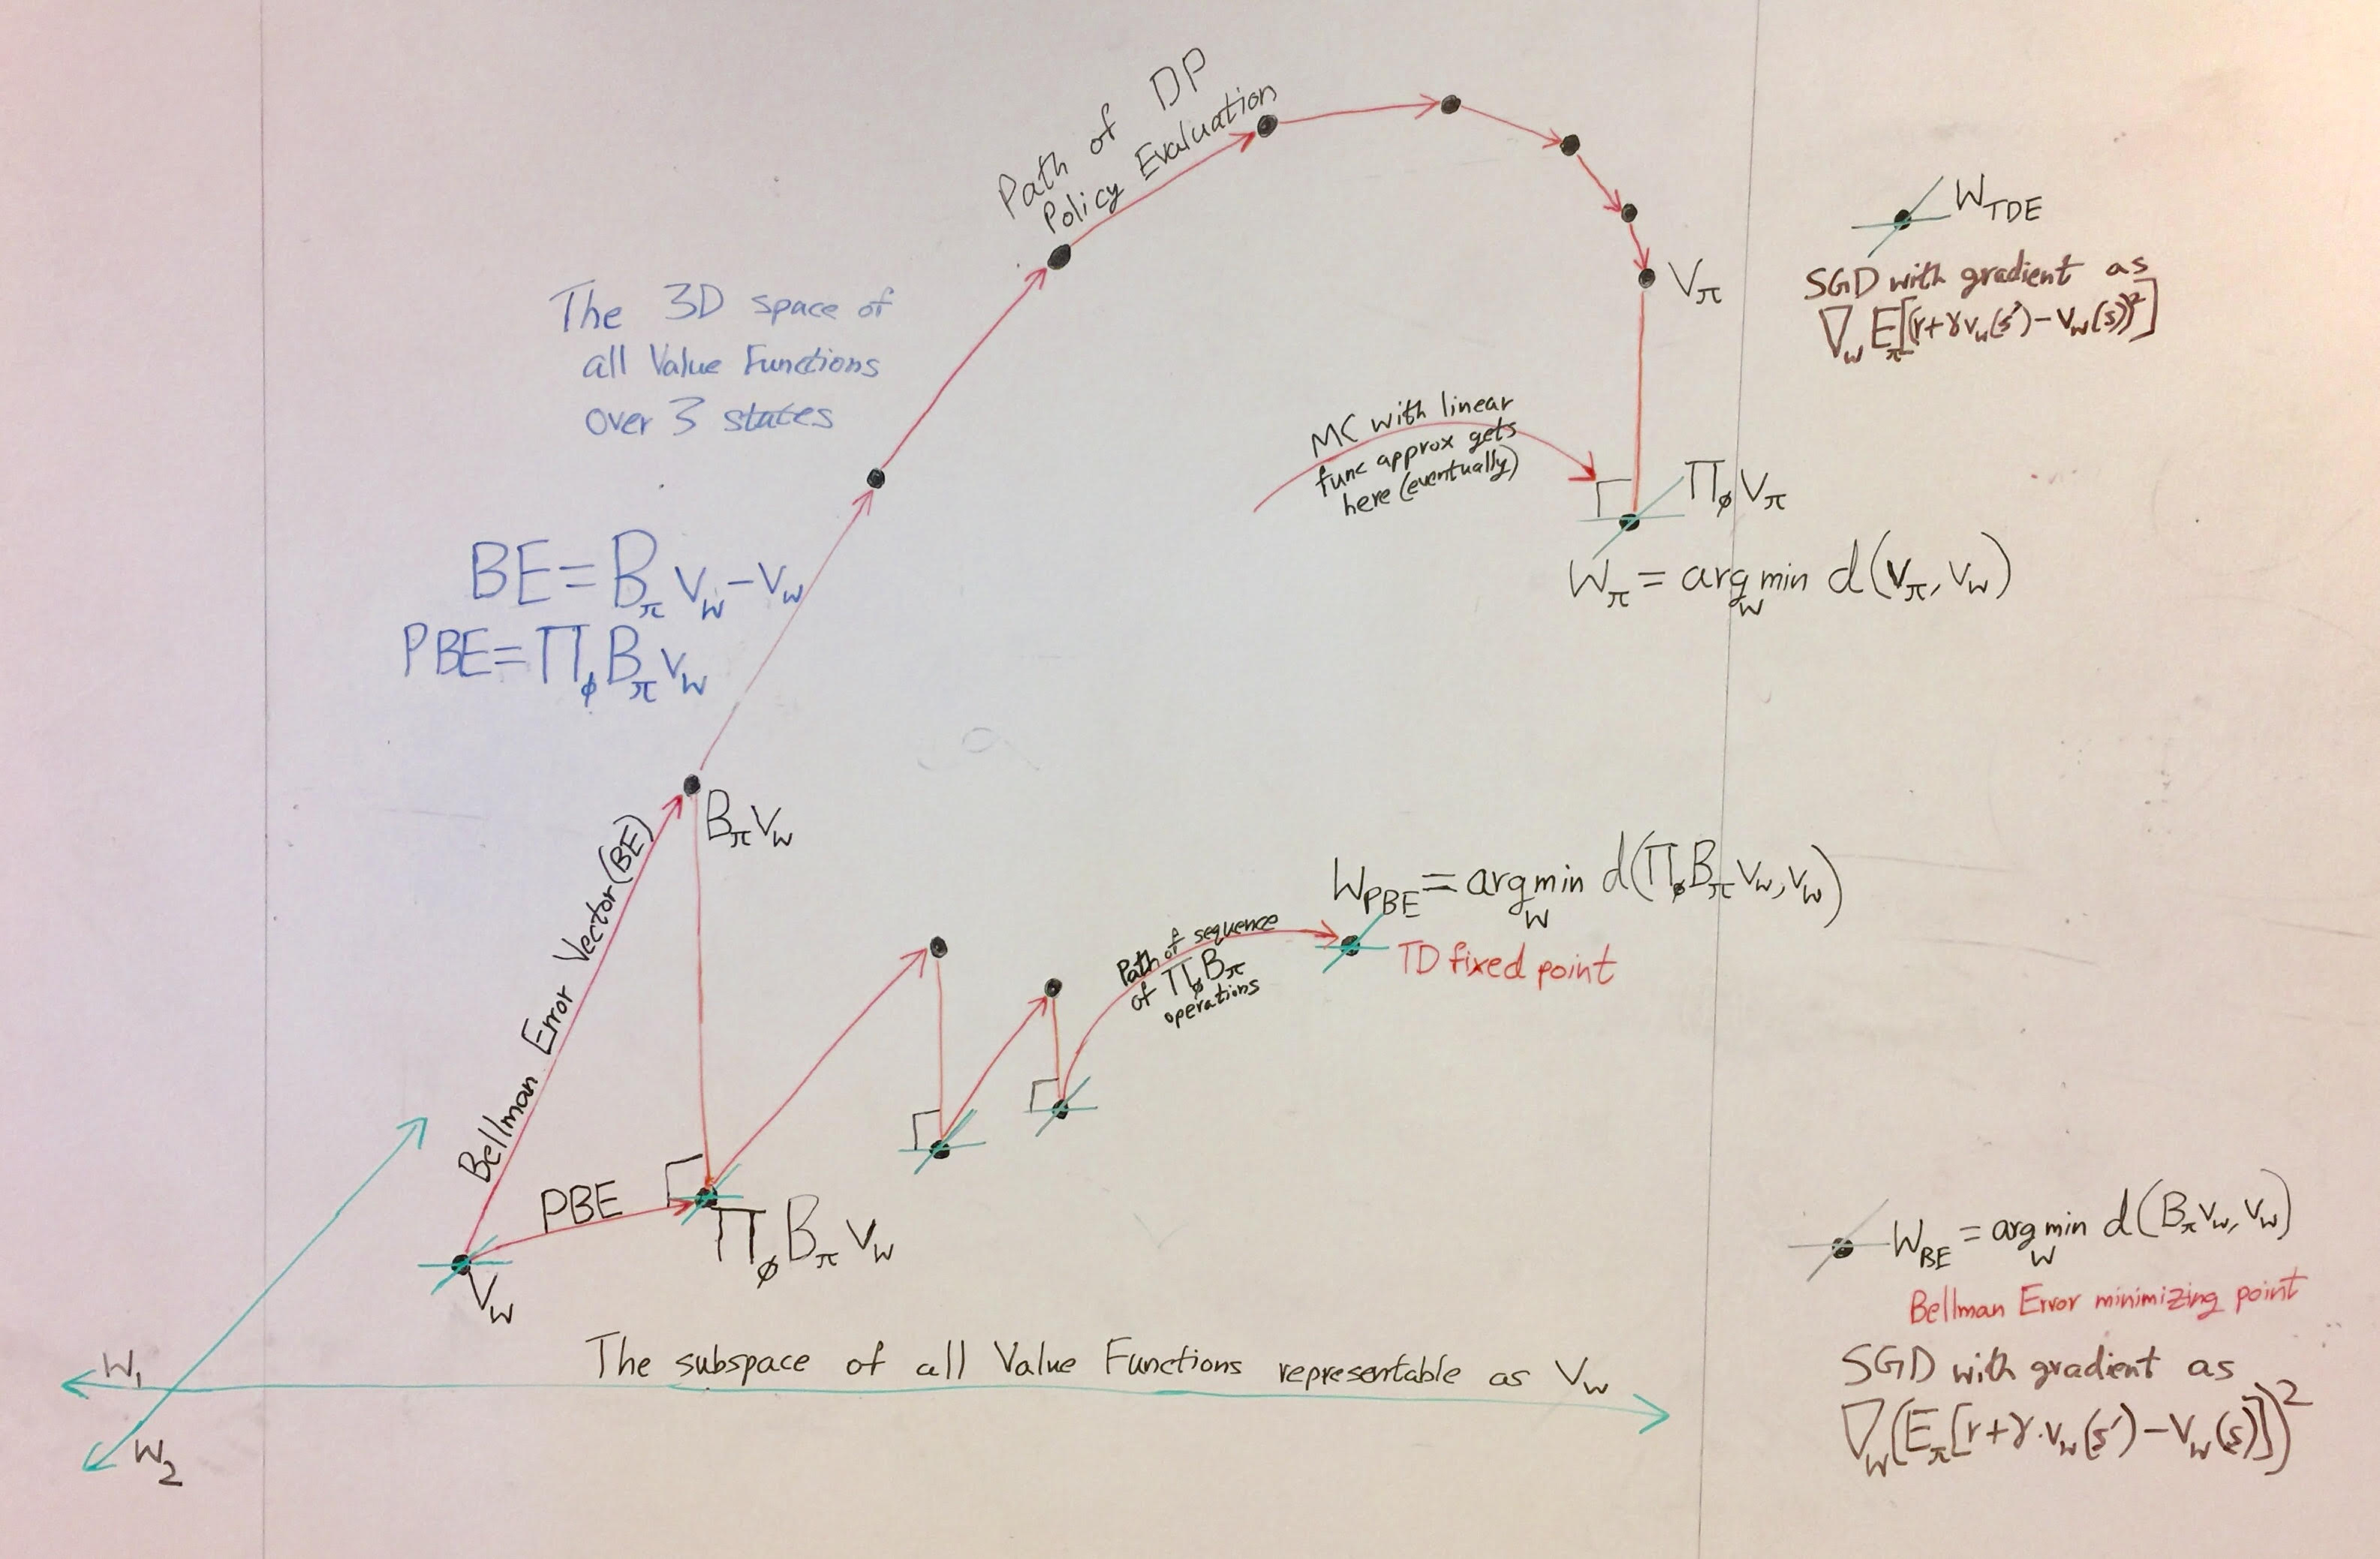
\includegraphics[scale=0.105]{VFGeometryImg.jpg}
\end{figure}
\end{frame}


\section{Solutions with Linear System Formulations}

\begin{frame}
\frametitle{Solution of $\bw_{BE}$ with a Linear System Formulation}
\begin{align*}
\bw_{BE} & = \argmin_\bw d(\vw, {\bf R}_{\pi} + \gamma {\bf P}_{\pi} \cdot \vw) \\
& = \argmin_\bw d(\bphi \cdot \bw, {\bf R}_{\pi} + \gamma {\bf P}_{\pi} \cdot \bphi \cdot \bw)\\
& = \argmin_\bw d(\bphi \cdot \bw - \gamma {\bf P}_{\pi} \cdot \bphi \cdot \bw, {\bf R}_{\pi} )\\
& = \argmin_\bw d((\bphi - \gamma {\bf P}_{\pi} \cdot \bphi) \cdot \bw, {\bf R}_{\pi} )\\
\end{align*}
This is a weighted least-squares linear regression of ${\bf R}_{\pi}$ versus $\bphi - \gamma {\bf P}_{\pi} \cdot \bphi$
with weights $\bmu$, whose solution is:
$$w_{BE} = ((\bphi - \gamma {\bf P}_{\pi} \cdot \bphi)^T \cdot \bd \cdot (\bphi - \gamma {\bf P}_{\pi} \cdot \bphi))^{-1} \cdot (\bphi - \gamma {\bf P}_{\pi} \cdot \bphi)^T \cdot \bd \cdot {\bf R}_{\pi}$$
\end{frame}

\begin{frame}
\frametitle{Solution of $\bw_{PBE}$ with a Linear System Formulation}
$\bphi \cdot {\bf w}_{PBE}$ is the fixed point of operator $\bpi \cdot \bb$. We know:
$$\bpi = \bphi \cdot (\bphi^T \cdot \bd \cdot \bphi)^{-1} \cdot \bphi^T \cdot \bd$$
$$\bb \bv = {\bf R}_{\pi} + \gamma {\bf P}_{\pi} \cdot \bv$$
Therefore,
$$\bphi \cdot (\bphi^T \cdot \bd \cdot \bphi)^{-1} \cdot \bphi^T \cdot \bd \cdot ({\bf R}_{\pi} + \gamma {\bf P}_{\pi} \cdot \bphi \cdot {\bf w}_{PBE}) = \bphi \cdot {\bf w}_{PBE}$$
Since columns of $\bphi$ are assumed to be independent (full rank),
\begin{align*}
(\bphi^T \cdot \bd \cdot \bphi)^{-1} \cdot \bphi^T \cdot \bd \cdot ({\bf R}_{\pi} + \gamma {\bf P}_{\pi} \cdot \bphi \cdot {\bf w}_{PBE}) & = {\bf w}_{PBE}\\
\bphi^T \cdot \bd \cdot ({\bf R}_{\pi} + \gamma {\bf P}_{\pi} \cdot \bphi \cdot {\bf w}_{PBE}) &= \bphi^T \cdot \bd \cdot \bphi \cdot {\bf w}_{PBE}\\
\bphi^T \cdot \bd \cdot (\bphi - \gamma {\bf P}_{\pi} \cdot \bphi) \cdot {\bf w}_{PBE} &= \bphi^T \cdot \bd \cdot {\bf R}_{\pi}\\ 
\end{align*}
This is a square linear system of the form ${\bf A} \cdot {\bf w}_{PBE} = {\bf b}$ whose solution is:
$${\bf w}_{PBE} = {\bf A}^{-1} \cdot {\bf b} = (\bphi^T \cdot \bd \cdot (\bphi - \gamma {\bf P}_{\pi} \cdot \bphi))^{-1} \cdot \bphi^T \cdot \bd \cdot {\bf R}_{\pi}$$
\end{frame}


\begin{frame}
\frametitle{Model-Free Learning of $\bw_{PBE}$}
\begin{itemize}
\item How do we construct matrix ${\bf A} = \bphi^T \cdot \bd \cdot (\bphi - \gamma {\bf P}_{\pi} \cdot \bphi)$ and vector ${\bf b} = \bphi^T \cdot \bd \cdot {\bf R}_{\pi}$ without a model?
\item Following policy $\pi$, each time we perform a model-free transition from $s$ to $s'$ getting reward $r$, we get a sample estimate of ${\bf A}$ and ${\bf b}$
\item Estimate of ${\bf A}$ is the outer-product of vectors $\phi(s)$ and $\phi(s) - \gamma \cdot \phi(s')$
\item Estimate of ${\bf b}$ is scalar $r$ times vector  $\phi(s)$ 
\item Average these estimates across many such model-free transitions
\item This algorithm is called Least Squares Temporal Difference (LSTD)
\item Alternative: Semi-Gradient Temporal Difference (TD) descent
\item This semi-gradient descent converges to ${\bf w}_{PBE}$ with weight updates:
$$\Delta w = \alpha \cdot (r + \gamma \cdot w^T \cdot \phi(s') - w^T \cdot \phi(s)) \cdot \phi(s)$$
\item $r + \gamma \cdot w^T \cdot \phi(s') - w^T \cdot \phi(s)$ is the TD error, denoted $\delta$
\end{itemize}
\end{frame}

\section{Residual Gradient TD}

\begin{frame}
\frametitle{Naive Residual Gradient Algorithm to solve for ${\bf w}_{TDE}$}
\begin{itemize}
\item We defined ${\bf w}_{TDE}$ as the vector in the $\bphi$ subspace that minimizes the expected square of the TD error $\delta$ when following policy $\pi$.
$${\bf w}_{TDE} = \argmin_{{\bf w}} \sum_{s \in \mathcal{S}} \bmu(s) \sum_{r,s'} prob_{\pi}(r, s'|s) \cdot (r + \gamma \cdot {\bf w}^T \cdot \phi(s') - {\bf w}^T \cdot \phi(s))^2$$
\item To perform SGD, we have to estimate the gradient of the expected square of TD error by sampling
\item The weight update for each sample in the SGD will be:
\begin{align*}
\Delta w & = - \frac{1}{2} \alpha \cdot \nabla_w (r + \gamma \cdot w^T \cdot \phi(s') - w^T \cdot \phi(s))^2\\
& = \alpha \cdot (r + \gamma \cdot w^T \cdot \phi(s') - w^T \cdot \phi(s)) \cdot (\phi(s) - \gamma \cdot \phi(s'))\\
\end{align*}
\item This algorithm (named {\em Naive Residual Gradient}) converges robustly, but not to a desirable place
\end{itemize}
\end{frame}

\begin{frame}
\frametitle{Residual Gradient Algorithm to solve for ${\bf w}_{BE}$}
\begin{itemize}
\item We defined ${\bf w}_{BE}$ as the vector in the $\bphi$ subspace that minimizes BE
\item But BE for a state is the expected TD error in that state
\item So we want to do SGD with gradient of square of expected TD error
\begin{align*}
\Delta w & = - \frac{1}{2} \alpha \cdot \nabla_w (\mathbb{E}_{\pi}[\delta])^2\\
& = - \alpha \cdot \mathbb{E}_{\pi}[r + \gamma \cdot w^T \cdot \phi(s') - w^T \cdot \phi(s)] \cdot \nabla_w \mathbb{E}_{\pi}[\delta]\\
& = \alpha \cdot (\mathbb{E}_{\pi}[r + \gamma \cdot w^T \cdot \phi(s')] - w^T \cdot \phi(s)) \cdot (\phi(s) - \gamma \cdot \mathbb{E}_{\pi}[\phi(s')])\\
\end{align*}
\item  This is called the {\em Residual Gradient} algorithm
\item Requires two independent samples of $s'$ transitioning from $s$
\item In that case, converges to ${\bf w}_{BE}$ robustly (even for non-linear approx)
\item But it is slow, and doesn't converge to a desirable place
\item Cannot learn if we can only access features, and not underlying states
\end{itemize}
\end{frame}

\section{Gradient TD}

\begin{frame}
\frametitle{Gradient TD Algorithms to solve for ${\bf w}_{PBE}$}
\begin{itemize}
\item For on-policy linear func approx, semi-gradient TD works
\item For non-linear func approx or off-policy, we need Gradient TD
\begin{itemize}
\item GTD: The original Gradient TD algorithm
\item GTD-2: Second-generation GTD
\item TDC: TD with Gradient correction
\end{itemize}
\item We need to set up the loss function whose gradient will drive SGD
\item ${\bf w}_{PBE} = \argmin_{\bf w} d(\bpi \bb \vw, \vw) = \argmin_{\bf w} d(\bpi \bb \vw, \bpi \vw)$
\item So we define the loss function (denoting $\bb \vw - \vw$ as $\bdel$) as:
$$\mathcal{L}({\bf w})  = (\bpi \bdel)^T \cdot \bd \cdot (\bpi \bdel) = \bdel^T \cdot \bpi^T \cdot \bd \cdot \bpi \cdot \bdel$$
$$=  \bdel^T \cdot (\bphi \cdot (\bphi^T \cdot \bd \cdot \bphi)^{-1} \cdot \bphi^T \cdot \bd)^T \cdot \bd \cdot  (\bphi \cdot (\bphi^T \cdot \bd \cdot \bphi)^{-1} \cdot \bphi^T \cdot \bd) \cdot \bdel$$
$$= \bdel^T \cdot (\bd \cdot \bphi \cdot (\bphi^T \cdot \bd \cdot \bphi)^{-1} \cdot \bphi^T) \cdot \bd \cdot  (\bphi \cdot (\bphi^T \cdot \bd \cdot \bphi)^{-1} \cdot \bphi^T \cdot \bd) \cdot \bdel$$
$$= (\bdel^T \cdot \bd \cdot \bphi) \cdot (\bphi^T \cdot \bd \cdot \bphi)^{-1} \cdot (\bphi^T \cdot \bd \cdot  \bphi) \cdot (\bphi^T \cdot \bd \cdot \bphi)^{-1} \cdot (\bphi^T \cdot \bd \cdot \bdel)$$
$$= (\bphi^T \cdot \bd \cdot \bdel)^T \cdot (\bphi^T \cdot \bd \cdot \bphi)^{-1} \cdot (\bphi^T \cdot \bd \cdot \bdel)$$
\end{itemize}
\end{frame}

\begin{frame}
\frametitle{TDC Algorithm to solve for ${\bf w}_{PBE}$}
We derive the TDC Algorithm based on $\nabla_{\bf w} \mathcal{L}({\bf w})$
$$\nabla_{\bf w} \mathcal{L}({\bf w}) = 2 \cdot (\nabla_{\bf w} (\bphi^T \cdot \bd \cdot \bdel)^T) \cdot (\bphi^T \cdot \bd \cdot \bphi)^{-1} \cdot (\bphi^T \cdot \bd \cdot \bdel)$$
Now we express each of these 3 terms as expectations of model-free transitions $s \stackrel{\mu}\longrightarrow (r,s')$, denoting $r + \gamma \cdot {\bw}^T \cdot \phi(s') - {\bw}^T \cdot \phi(s)$ as $\delta$
\begin{itemize}
\item $\bphi^T \cdot \bd \cdot \bdel = \mathbb{E}[\delta \cdot \phi(s)]$
\item $\nabla_{\bf w} (\bphi^T \cdot \bd \cdot \bdel)^T = \nabla_{\bf w} (\mathbb{E}[\delta \cdot \phi(s)])^T = \mathbb{E}[(\nabla_{\bf w} \delta) \cdot \phi(s)^T] = \mathbb{E}[(\gamma \cdot \phi(s') - \phi(s)) \cdot \phi(s)^T]$
\item $\bphi^T \cdot \bd \cdot \bphi = \mathbb{E}[\phi(s) \cdot \phi(s)^T]$
\end{itemize}
Substituting, we get:
$$\nabla_{\bf w} \mathcal{L}({\bf w}) = 2 \cdot  \mathbb{E}[(\gamma \cdot \phi(s') - \phi(s)) \cdot \phi(s)^T] \cdot \mathbb{E}[\phi(s) \cdot \phi(s)^T]^{-1} \cdot \mathbb{E}[\delta \cdot \phi(s)]$$
\end{frame}

\begin{frame}
\frametitle{Weight Updates of TDC Algorithm}
$$\Delta w  = - \frac {1} {2} \alpha \cdot \nabla_{\bf w} \mathcal{L}({\bf w})$$
$$ = \alpha \cdot \mathbb{E}[(\phi(s) - \gamma \cdot \phi(s')) \cdot \phi(s)^T] \cdot \mathbb{E}[\phi(s) \cdot \phi(s)^T]^{-1} \cdot \mathbb{E}[\delta \cdot \phi(s)]$$
$$ = \alpha \cdot (\mathbb{E}[\phi(s) \cdot \phi(s)^T] - \gamma \cdot \mathbb{E}[\phi(s') \cdot \phi(s)^T]) \cdot \mathbb{E}[\phi(s) \cdot \phi(s)^T]^{-1} \cdot \mathbb{E}[\delta \cdot \phi(s)]$$
$$ = \alpha \cdot (\mathbb{E}[\delta \cdot \phi(s)] - \gamma \cdot \mathbb{E}[\phi(s') \cdot \phi(s)^T] \cdot \mathbb{E}[\phi(s) \cdot \phi(s)^T]^{-1} \cdot \mathbb{E}[\delta \cdot \phi(s)])$$
$$ = \alpha \cdot (\mathbb{E}[\delta \cdot \phi(s)] - \gamma \cdot \mathbb{E}[\phi(s') \cdot \phi(s)^T] \cdot \theta)$$

\vspace*{2mm}

where $\theta = \mathbb{E}[\phi(s) \cdot \phi(s)^T]^{-1} \cdot \mathbb{E}[\delta \cdot \phi(s)]$ is the solution to a weighted least-squares linear regression of $\bb \bv - \bv$ against $\bphi$, with weights as $\mu_{\pi}$.

\vspace*{3mm}

{\bf Cascade Learning: Update both $w$ and $\theta$} ($\theta$ converging faster)
\begin{itemize}
\item $\Delta w = \alpha \cdot \delta \cdot \phi(s)  - \alpha \cdot \gamma \cdot \phi(s') \cdot (\theta^T \cdot \phi(s))$
\item $\Delta \theta = \beta \cdot (\delta - \theta^T \cdot \phi(s)) \cdot \phi(s)$
\end{itemize}
Note: $\theta^T \cdot \phi(s)$ operates as estimate of TD error $\delta$ for current state $s$

\end{frame}
\end{document}
